Luego del proceso de anotación y corrección de lemas y etiquetas gramaticales,
se extrajeron algunas métricas de resumen y se realizaron gráficos con el fin de
comprender qué distribución presentaban dichas etiqutas utilizadas y cuántos de los
datos etiquetdados de forma automática requirieron alguna corrección, ya fuera en el
lema asignado, ya en la etiqueta gramatical predicha.
\par
En total, se revisaron 8324 anotaciones\footnote{Cada anotación está dada por
la ocurrencia \textit{cruda} de la palabra, la etiqueta (o etitquetas, si el modelo
predijo más de una posible) de esa palabra en los discursos en los que fue vista y el
lema (o lemas, si se predijo más de uno) para esa palabra en tales contextos.}.
De ellas, se despreciaron 211 cadenas de caracteres ($1.86\percentsign$)
\footnote{Remitirse a \ref{appendix-annotation} para un detalle de las palabras
despreciadas.}. De las palabras que se persistieron para el análisis,
el $12.35\percentsign$ requirió una corrección en la etiqueta gramatical.
En la mayoría de estos casos ($71\percentsign$), el modelo predijo más de una etiqueta
posible para determinada palabra y una de ellas resultó ser la adecuada, solo que no
fue predicha de forma consistente. En el resto de los casos ($29\percentsign$)
el modelo no fue capaz de identificar la etiqueta adecuada en ningún caso.
Respecto de los lemas, el $20.4\percentsign$ de las palabras debió ser corregida
y, de estas, el $27.8\percentsign$ de las correcciones fueron casos en los que el
modelo predijo al menos una vez el lema correcto, pero no hizo tal predicción de
forma consistente, y el $72.2\percentsign$ fueron casos en los que el modelo
no logró predecir el lema correcto en ninguna situación.
\par
Al final del procedimiento se obtuvo un conjunto de 4889 \textit{tokens} únicos,
donde la unicidad hace referencia al lema y a la etiqueta gramatical asignada.
En el análisis exploratorio realizado para la descripción de los datos, la unicidad
de los \textit{tokens} estaba dada por la igualdad en la secuencia de caracteres
en la ocurrencia efectiva de la palabra: allí `suma' se considera
una sola vez, independientemente de si, en sus distintas ocurrencias, refiere al
verbo (en la tercera persona singular del verbo `sumar') o al nombre
(\textit{``acción y efecto de sumar''}\footnote{\Citeauthor{rae23diccionario}.}). Al
agrupar los \textit{tokens} por lemas y etiqueta gramatical, estas dos
ocurrencias son consideradas por separado, dado que se toma en cuenta
`suma (\textit{NOUN})' y `sumar (\textit{VERB})'. La figura
\ref{fig-distrib-unique-tokens} refleja el contraste en la longitud de
discursos al ser medidos con ambos enfoques. Allí se puede observar que,
como es deesperar, las longitudes medidas considerando lemas y etiquedas
\textit{POS} reflejan valores menores.

\begin{figure}[h!]
\centering
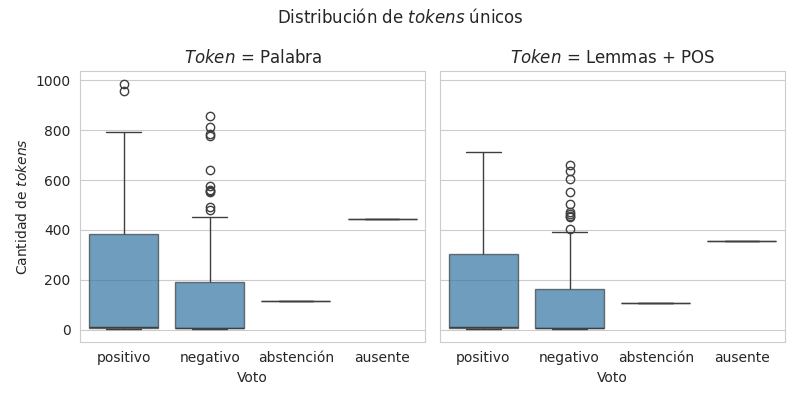
\includegraphics[scale=0.45]{../visualizations/distrib_tokes_vs_lemma_pos/distrib_tokens_vs_lemma_pos.png}
\caption{Distribución \textit{tokens} únicos aplicando distintos criterios de unicidad.}
\label{fig-distrib-unique-tokens}
\end{figure}